\begin{titlepage}
\newgeometry{margin=0.95in}
\thispagestyle{empty}

\begin{center}
{\large University of Rochester\\}
{\normalsize Warner School of Education\\[0.35in]}

{\color{PrimaryRed}\rule{\textwidth}{1.4pt}}\\[0.22in]
{\Huge\bfseries Literacy as Power:\\[0.08in] Communication Access,\\[0.08in] Neurodivergence, and Social Justice\\[0.08in] in STEM Education}\\[0.18in]
{\Large Critical Literacy Journal}\\[0.22in]
{\color{PrimaryRed}\rule{0.78\textwidth}{0.7pt}}\\[0.32in]

\colorbox{SoftBlue}{%
\parbox{0.88\textwidth}{%
\centering\vspace{0.12in}
\textbf{Communication Access as Literacy, Power, and Educational Justice}\\[0.05in]
A literacy and social justice analysis of classroom communication, disciplinary language, accommodation systems, and institutional literacy.
\vspace{0.12in}
}%
}
\end{center}

\vspace{0.25in}

\begin{center}
\renewcommand{\arraystretch}{1.15}
\setlength{\tabcolsep}{4pt}
\begin{tabular}{>{\bfseries\RaggedLeft}p{1.65in} p{4.9in}}
Student & Piter Zacari Garcia Bautista \\
Course & EDU498: Literacy Learning as Social Practice \\
Assignment & Literacy as Power: Bridging Social Justice and Critical Communication \\
Focus & Communication access injustice for neurodivergent and chronically ill students in STEM education \\
Present-Day Connection & Universal Design for Learning / CAST UDL Guidelines 3.0 \\
Submission Date & June 2026 \\
\end{tabular}
\end{center}

\vspace{0.25in}

\begin{center}
\begin{minipage}{0.95\textwidth}
\itshape
This journal uses a BIO/STEM communication-access case as an evidence site for a broader literacy and social justice argument. It examines how classroom communication, disciplinary terminology, accommodations, and institutional pathways can determine whether students are understood, supported, and allowed to participate with dignity.

\vspace{0.22in}

\scriptsize\centering\textbf{Working draft note:} This version uses the visual structure of the Minecraft identity mini-unit template. Final revision should add final screenshots, tighten citations to course readings, and polish transitions before submission.
\end{minipage}
\end{center}

\restoregeometry
\end{titlepage}
\clearpage
\onehalfspacing

\section*{The Bridge}

\begin{wrapfigure}{r}{0.43\textwidth}
    \vspace{-4em}
    \centering
    
\includegraphics[
        width=0.43\textwidth,
        height=0.43\textheight,
        keepaspectratio
    ]{images/real_pain_real_injustice.png}
    % \vspace{-0.5em}
    {\scriptsize\textit{Figure 1. A visual map of communication harm, institutional rigidity, and the emotional burden created by inaccessible teaching design.}\par}
    \vspace{-1.5em}
\end{wrapfigure}

This paper dives into the intersection of literacy and social justice by showing how communication systems can empower or exclude communities. In my BIO/STEM communication-access case, course literacy did not only mean reading and writing but being able to decode requirements, accommodations, grading language, single-mode directions, team expectations, scientific communication norms, and institutional pathways. If a teacher uses their authority, knowledge, or influence to communicate through one-size-fits-all expectations, they intentionally or unintentionally exclude neurodivergent, ill, disabled, culturally and linguistically diverse, trauma-impacted, and otherwise vulnerable students.

The paper uses a documented adult learning experience/pain as a case for analyzing a larger social justice problem: communication access injustice in education, centering the following question: if an adult graduate student with technical knowledge, documentation habits, advisor support, and self-advocacy skills can still be harmed by purposefully designed inaccessible communication, \textit{what happens to children and younger students who cannot defend themselves yet?}


\section*{Communication Access as a Social Justice Issue -- Research Findings}

% \subsection*{Identify the Topic}
\begin{wrapfigure}{l}{0.5\textwidth}
\vspace{-2em}
\centering
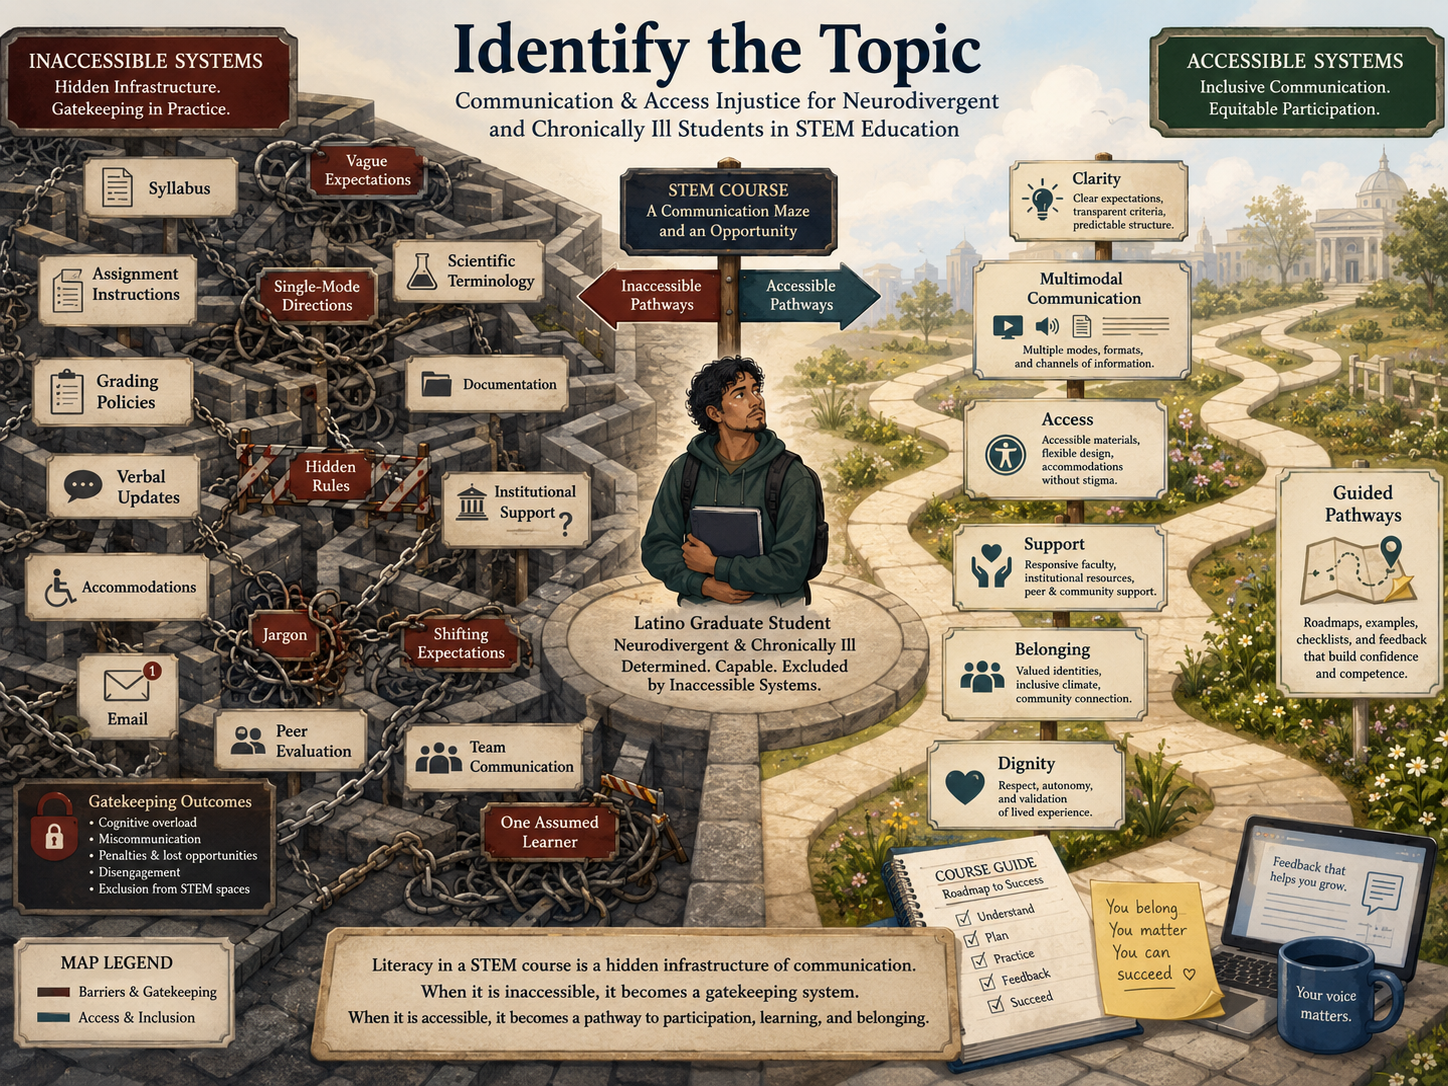
\includegraphics[
width=0.5\textwidth,
height=0.5\textheight,
keepaspectratio
]{images/identifying_the_real_topic.png}
% ```
% \vspace{-0.5em}
{\scriptsize\textit{Figure 2. Identifying the real topic: a visual map showing how communication breakdowns, institutional rigidity, and inaccessible teaching design can shift the burden onto students rather than addressing the system-level barriers that shape learning.}\par}
\vspace{-1.5em}
% ```
\end{wrapfigure}

The issue I am focusing on is \textit{communication and access injustice for neurodivergent and chronically ill students in STEM education}. This issue sits directly at the intersection of literacy and social justice because literacy is not only the ability to read and write words. In school, literacy also means being able to access, decode, interpret, and respond to the communication systems that organize learning.

In a STEM classroom, those communication systems include the syllabus, assignment instructions, clear grading policies, verbal updates, accommodation procedures, email exchanges, evaluations, expectations, team communication, tools, scientific terminology, documentation, and institutional support pathways. \textit{A student is not only learning bioinformatics, computer/data science, but also learning how to navigate the course itself.}

When those systems are clear, stable, accessible, and multimodal, literacy can empower students. It can help them understand expectations, ask better questions, use accommodations, collaborate with peers, and show what they know. However, when those systems are vague, single-mode, inconsistent, hidden, or built around one assumed kind of learner, literacy becomes a gatekeeping system. Students who don't process, remember, communicate, or participate in that way can be misread as difficult, unprepared, irresponsible, or less capable.

% \newpage
That is why this issue is about social justice; a teacher's communication choices decide who gets access to learning and who has to fight to be understood. Even when a teacher does not intend harm, their authority, disciplinary knowledge, and classroom structure can exclude students if communication is designed for only one kind of body, brain, language background, pace, memory system, or emotional response.

The BIO/STEM evidence I gathered for this paper documents this issue through my own experience in a bioinformatics course. The larger issue observed is how inaccessible communication affects neurodivergent, ill, disabled, culturally and linguistically diverse, trauma-impacted, anxious, depressed, and otherwise vulnerable students across educational settings.

\subsection*{Why This Issue Matters}

\begin{wrapfigure}{r}{0.4\textwidth}
\vspace{-6em}
\centering
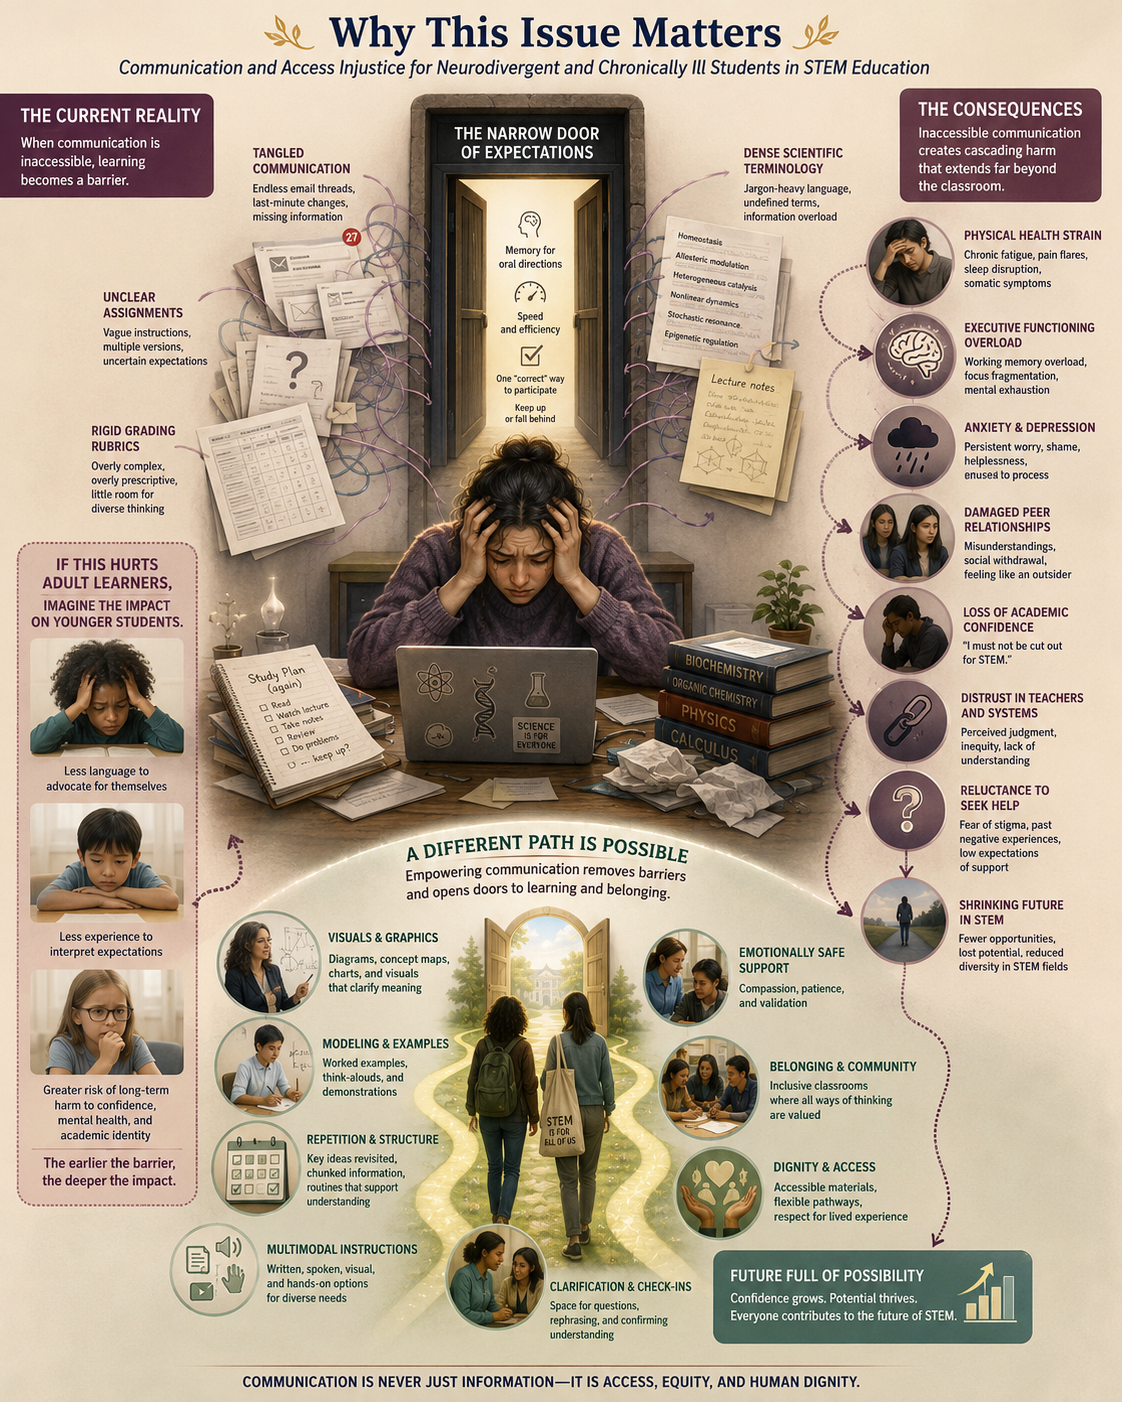
\includegraphics[
width=0.4\textwidth,
height=0.4\textheight,
keepaspectratio
]{images/why_this_issue_matters.png}
% `% \vspace{-0.5em}
{\scriptsize\textit{Figure 3. A visual explanation of how inaccessible communication, rigid institutional responses, and narrow interpretations of student behavior can turn learning barriers into personal blame instead of prompting more humane, responsive design.}\par}
\vspace{-1.5em}
%`
\end{wrapfigure}


Communication determines access. Therefore, if a student cannot reliably find, understand, remember, or clarify the language of a course, then the student cannot fully access the learning the course claims to offer. Inaccessible communication can affect far more than grades. It can affect physical health, executive functioning, mental health, peer relationships, academic confidence, trust in teachers, willingness to seek help, identity as a capable learner, and future participation in STEM. This is a historically relevant issue; schools have often organized learning around a narrow image of the successful student: someone who can sit still, remember oral instructions, use dominant academic language, respond quickly, communicate calmly under stress, tolerate ambiguity, and perform knowledge in approved formats. Students who do not match that image are often misread. Neurodivergent students may be seen as careless, disruptive, lazy, too intense, or disorganized. Chronically ill students may be seen as unreliable. Culturally and linguistically diverse, multilingual students may be perceived as less prepared when the real issue is institutional language. Students with trauma, depression, or anxiety may be seen as avoidant or difficult when the communication environment itself feels threatening.

This becomes especially urgent in STEM because STEM courses can confuse rigor with rigidity. \textit{A course can be intellectually demanding without being inaccessible}. But when instructors treat ambiguity, memory for oral directions, single-mode output, public correction, or emotional toughness as evidence of rigor, students with access needs are quietly sorted out. The problem is that access should be part of rigor. This issue also matters in my field of study because bioinformatics and computer science are deeply literate fields. They require students to read scientific instructions, interpret computational tasks, understand data files, communicate through code, document processes, coordinate digital teamwork, translate technical thinking into reports, and navigate institutional policies. If a course treats these literacies as obvious instead of teachable and accessible, it can exclude students even when they have the intellectual capacity to do the work.

The local community connection is another important aspect in using literacy as power. In Literacy Learning as Social Practice and in my teaching placement, I have seen how much students, especially children, rely on clear communication, modeling, visuals, repetition, embodied practice, peer explanation, and emotionally safe clarification. Children often cannot document harm, email advisors, cite accommodations, or explain that a classroom expectation is inaccessible by design. \textit{They may simply shut down, act out, become overwhelmed, or internalize that they are the problem.} If an adult graduate student with documentation habits, technical expertise, advisor support, and self-advocacy skills can still be harmed by inaccessible communication, then \textit{children and less-resourced students are at even greater risk}. They shouldn't need to be experts in institutional navigation before they are allowed to be learners.

\subsection*{Relevant Sources and Evidence Scope}

\begin{wrapfigure}{r}{0.6\textwidth}
\vspace{-5em}
\centering
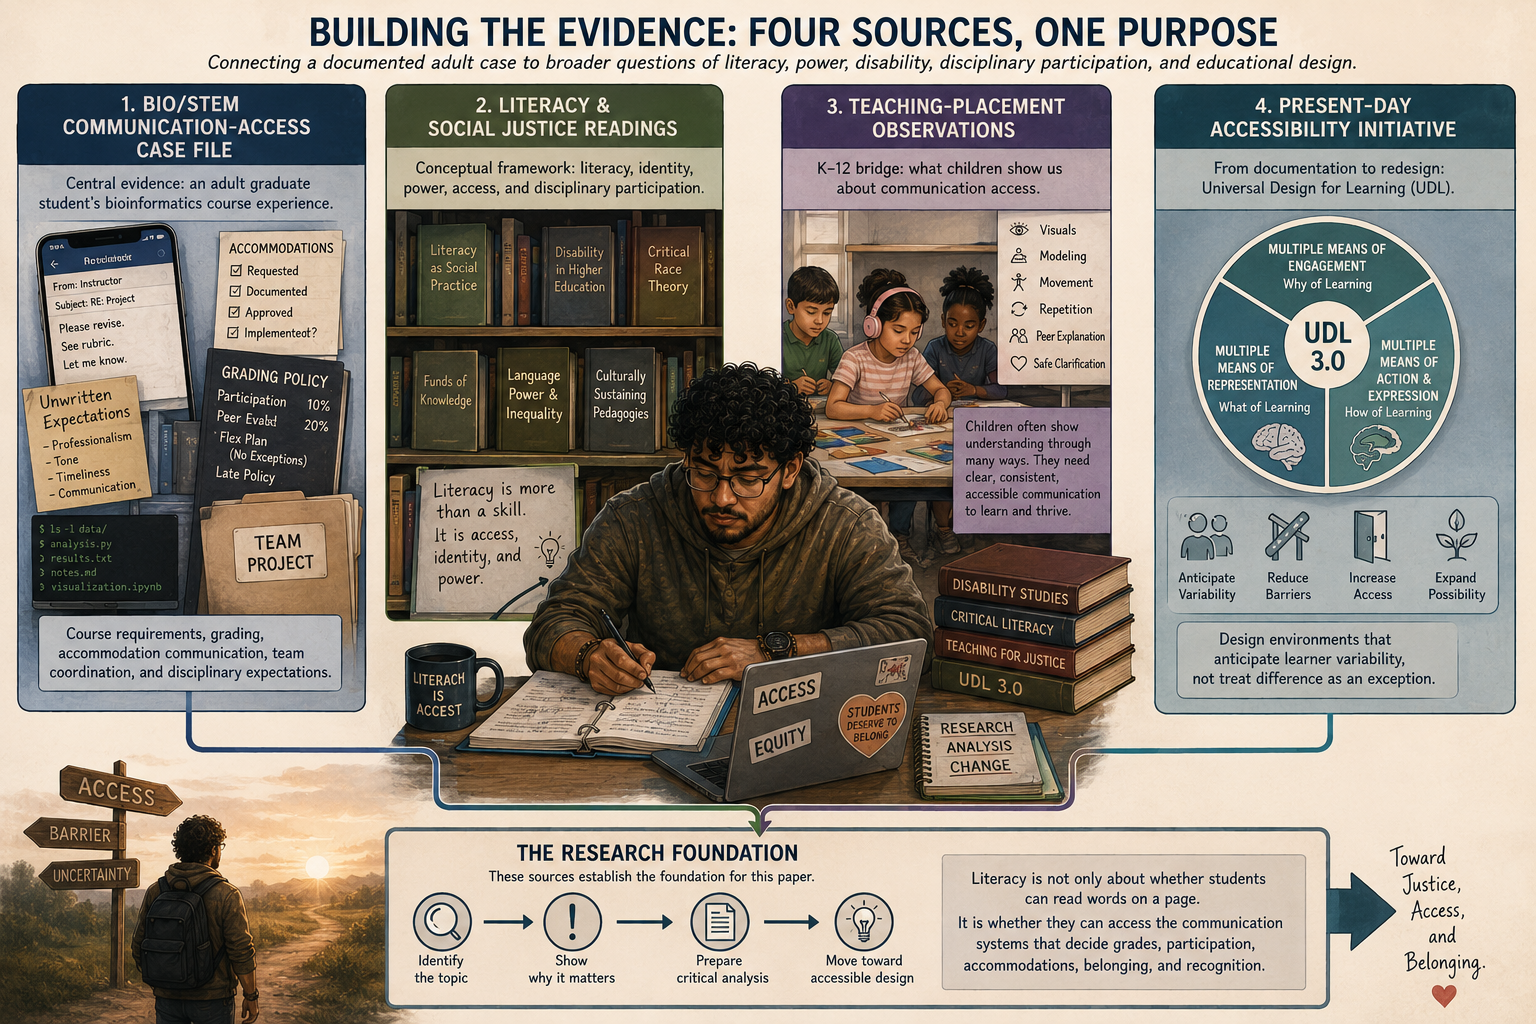
\includegraphics[
width=0.6\textwidth,
height=0.6\textheight,
keepaspectratio
]{images/building_the_evidence.png}
% `% \vspace{-0.5em}
{\scriptsize\textit{Figure 4. A visual map showing how repeated communication barriers, documented interactions, student effort, and institutional responses create a pattern of evidence that shifts the issue from an isolated misunderstanding to a systemic access concern.}\par}
\vspace{-1.5em}
%`
\end{wrapfigure}

The research for this paper draws from four sources of evidence: a curated BIO/STEM communication-access case file, literacy and social justice course readings, teaching-placement observations, and a present-day accessibility initiative. Together, these sources connect a documented adult learning experience to broader questions of literacy, power, disability, disciplinary participation, and educational design.

My \textit{communication-access} documented cases serve as the central evidence source for the adult case. It brings together course communication, selected classroom and team records, advisor-supported institutional navigation, and examples of scientific and technical communication. My evidence focuses on how access barriers emerged through the course requirements, grading procedures, accommodation communication, team coordination, and disciplinary expectations. The examples include undocumented or unstable procedural expectations, grading language that required interpretation beyond the written policy, health-related communication that increased the burden on any chronically ill student, accommodation procedures experienced through \textit{unethical, borderline illegal, compliance limits} rather than inclusive design, collaborative project expectations without sufficient communication norms, and specialized scientific terminology treated as self-evident rather than explicitly supported.

The \textit{literacy and social justice readings} provide the conceptual framework for interpreting the BIO/STEM evidence. These readings position literacy as more than a technical skill. They connect literacy to identity, disciplinary participation, criticality, language power, access, and joy. This framework matters because the paper is not only asking what happened in one course. It is asking \textit{how classroom communication can position students as capable or incapable, included or excluded, legitimate or difficult.}

\newpage
The \textit{teaching-placement observations} provide the K--12 bridge. They connect the adult BIO/STEM case to children who often demonstrate understanding through action, tools, collaboration, movement, design, peer explanation, and repeated guided practice. This matters because children usually cannot document harm, email advisors, cite accommodations, or explain that an expectation is inaccessible by design. My teaching placement has shown me why communication access must be designed before harm occurs.

The \textit{present-day accessibility initiative}, Universal Design for Learning (UDL), especially CAST UDL Guidelines 3.0, supports the move from documentation to redesign. This initiative connects the issue to the present, but it is also part of the research direction because it offers a current framework for designing learning environments that anticipate learner variability rather than treating difference as an exception \citep{cast2024udl}.

Together, these sources establish the research foundation for the paper. They helped identify the topic, show why it matters, and prepare the critical analysis that follows: literacy is not only about whether students can read words on a page. Literacy is whether students can access the communication systems that decide grades, participation, accommodations, belonging, and recognition.

% \newpage
\section*{Literacy as Communication Power -- A Critical Analysis}

\begin{wrapfigure}{l}{0.55\textwidth}
\vspace{-3em}
\centering
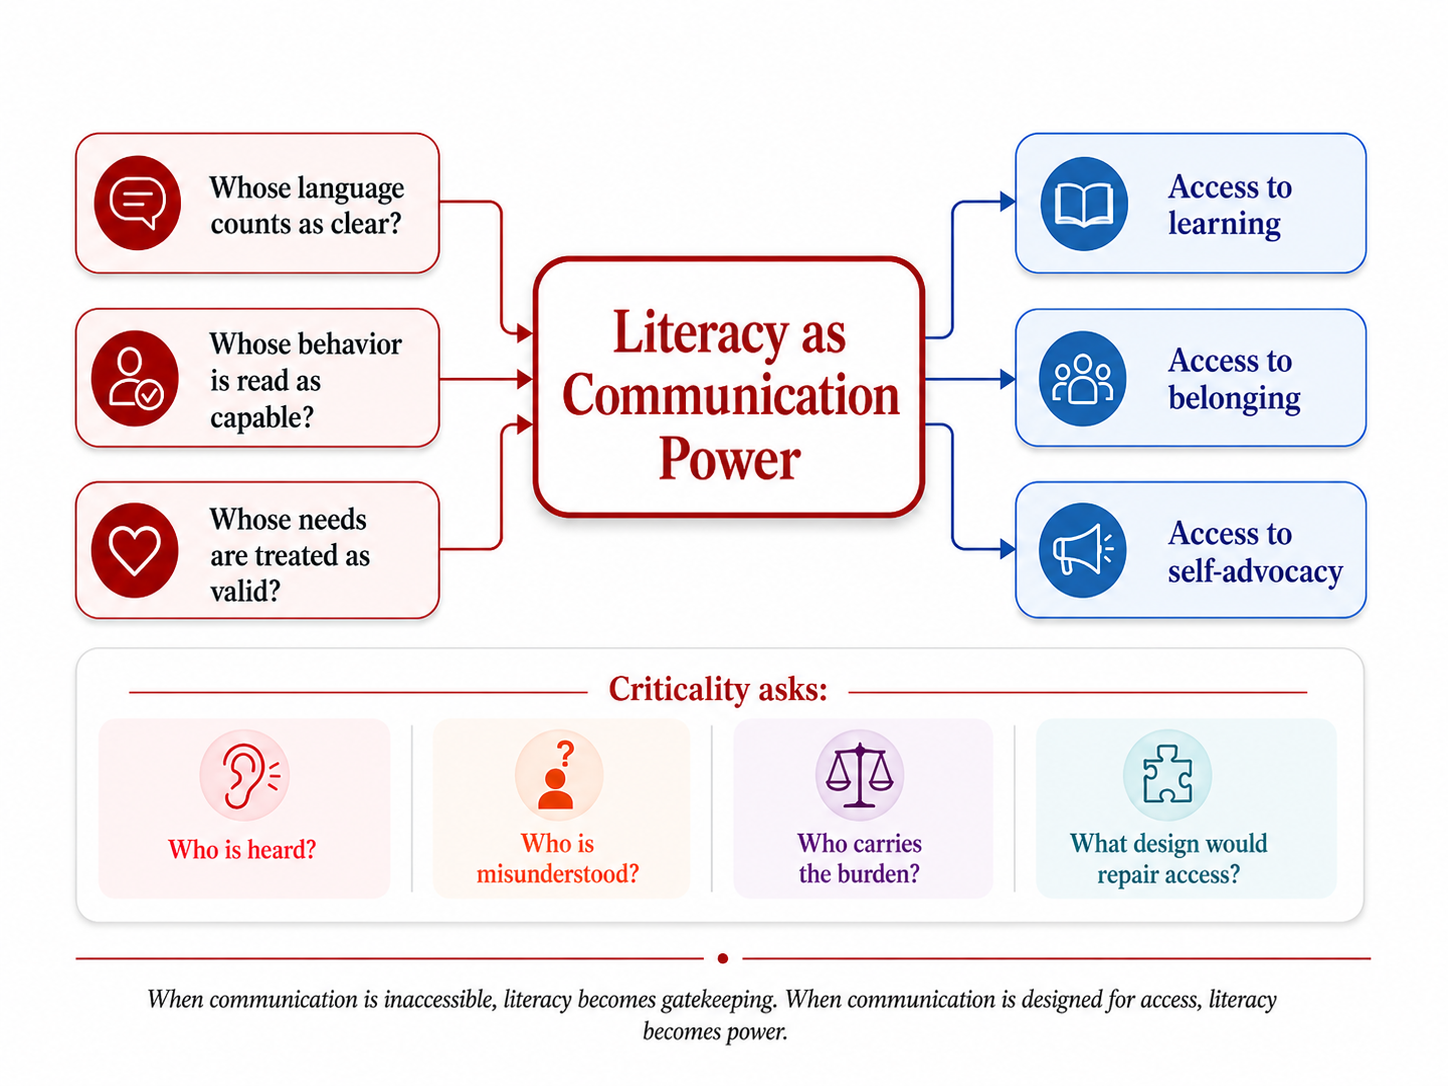
\includegraphics[
width=0.55\textwidth,
height=0.55\textheight,
keepaspectratio,
trim=1.2cm 0.4cm 1.2cm 0.3cm,
clip
]{images/literacy_as_communication_power.png}

{\scriptsize\textit{Figure 5. This visual shows how literacy is shaped by whose language is recognized, whose behavior is interpreted as capable, and whose access needs are treated as valid. It reframes communication as a power issue and not as an individual student responsibility.}\par}
\vspace{-2em}
\end{wrapfigure}

Literacy shapes how communication access injustice is understood because the issue is often obscured by neutral-sounding language. Words like \textit{rigor}, \textit{professionalism}, \textit{participation}, \textit{responsibility}, \textit{reasonable accommodation}, and \textit{student expectations} can appear fair on the surface while still placing uneven burdens on students whose bodies, brains, languages, or trauma histories do not match the assumed classroom norm. In this way, literacy does not simply communicate a social justice issue; it can also disguise the issue.

In my BIO/STEM communication-access evidence, the problem is not only that individual instructions were unclear. The deeper issue is that course communication operated through a set of literacy demands that were treated as obvious: knowing which expectations were official, knowing how to interpret grading language, knowing when a classroom direction carried the force of policy, knowing how to translate illness into made-up  institutional procedure, knowing how to use accommodations without appearing difficult, and knowing how to take teachers' responsibility to maintain overall team participation while managing multiple health conditions. These are not minor communication details but access conditions.

\subsection*{Language, Tone, and Authority}

The language of a course carries institutional power because students rarely meet course communication as equals. \textit{A professor's wording can determine what counts as responsible, late, complete, professional, respectful, or valid}. When expectations are communicated through unstable, single-mode, or implied channels, the student must do more than complete the assignment. The student must interpret the system. The same sentence can have different consequences depending on who receives it. A student without health barriers may experience an unclear requirement as an inconvenience. A neurodivergent student may experience it as an executive-function crisis. An ill student may experience it as another demand layered on top of symptoms, medication effects, and disclosure fatigue. \textit{A child may not experience it as communication ambiguity at all; they may simply experience shame, shutdown, or punishment.}

My BIO/STEM evidence shows clearly how \textit{communication becomes exclusionary while being framed as ordinary course management}. Procedural expectations communicated through \textit{unofficial modes} became inaccessible for neurodivergent students that rely on stable written records. Grading language requiring interpretation beyond the written policy \textit{turned assignments into policy decoding}. Health-related communication shifted responsibility back to the student, even during moments when the student had the least capacity. Accommodation language became a \textit{compliance checkpoint rather than an access design}. Team communication became another barrier when collaboration took place without explicit norms. The issue, then, was not whether communication exists. \textit{The issue was whether communication was accessible}, stable, interpretable, and humane.

\subsection*{Terminology as Access or Exclusion}

Specific terms can exclude students when they are used as if everyone shares the same institutional, disciplinary, or disability literacy. In this case, terms such as \textit{Flex Plan}, \textit{DSO}, \textit{Ombuds}, \textit{peer evaluation}, \textit{formative feedback}, \textit{participation}, \textit{professional communication}, and \textit{rigor} are not simple vocabulary words. They are gatekeeping terms when students are expected to understand their consequences without explicit explanation. Scientific and technical terminology can create a similar barrier. In bioinformatics and computer science, students are expected to understand not only concepts, but also formats, workflows, documentation practices, computational tools, and disciplinary conventions. Specialized language is necessary in STEM, but it becomes exclusionary when it is treated as self-evident rather than taught, modeled, or connected to clear expectations. This distinction matters. The goal is not to remove specialized language from STEM but to make specialized language accessible. \textit{Students should be able to learn the language of the field without also having to decode hidden classroom rules, unclear grading procedures, or institutional processes during moments of crisis}.

\subsection*{Audience Literacy and Unequal Burden}

Different audiences bring different kinds of literacy to this issue. A graduate student may have advanced scientific literacy but still struggle with institutional ambiguity, accommodation procedures, or unclear grading language. A neurodivergent student may have strong analytical literacy but need stable written expectations, predictable channels, and explicit sequencing. An ill student may understand the work but need communication structures that account for variable capacity. A culturally and linguistically diverse or multilingual student may understand concepts but be excluded by unexplained institutional language or dominant academic tone. A student with trauma, anxiety, or depression may experience public correction, uncertainty, or conflict as a threat rather than feedback.

Children are at even greater risk because they usually lack the institutional language adults can use to defend themselves. They may not know how to say that a classroom expectation is inaccessible, that a direction was too vague, that they needed a visual model, that public correction made them shut down, or that they understood the idea but could not perform it in the required format. Instead, their behavior may be misread. \textit{They may be labeled inattentive, oppositional, unmotivated, careless, or disruptive.} This is where my BIO/STEM evidence becomes a warning. If an adult with documentation practices, technical expertise, advisor support, and self-advocacy skills can still be harmed by inaccessible communication, then children and less-resourced students face even greater danger. They are less likely to have the language, power, or protection needed to challenge the system. For them, \textit{communication access cannot be optional, and must be designed before harm occurs}.

\subsection*{Literacy as the Mediator of Social Justice}

The course readings on literacy, identity, disciplinary learning, and criticality help explain why this is a social justice issue. Literacy is not neutral; it can recognize students as capable, or it can make their needs appear excessive. It can invite participation, or it can make participation dependent on decoding hidden rules. \textit{It can support identity, or it can force students to mask, over-document, or repeatedly justify their existence in the classroom}. Through this lens, communication access is part of educational justice. A classroom that values only one way of processing, remembering, speaking, writing, participating, or demonstrating knowledge is not rigorous in a meaningful sense. It is selective; \textit{it rewards students who fit the expected literacy profile and penalizes students whose literacy appears in different forms}. A more just classroom does not lower standards but clarifies them, it makes expectations visible. It teaches disciplinary language explicitly and repeats important changes in writing. \textit{It treats accommodations as a starting point for design}, recognizing that students demonstrate understanding through multiple literacies: written, oral, visual, technical, embodied, collaborative, emotional, and institutional. This is the bridge to the recommendations that follow. The solution is not only better individual kindness. The solution is better communication design. Literacy can exclude, but it can also empower when educators design systems that allow students to understand expectations, access support, participate with dignity, and show what they know without having to break themselves first.
